% IEEE conference summary of the MSc dissertation
% "Fast response MPPT charger for the Técnico Solar Boat"
% Template filename follows the IEEE conference template (conference_101719).
\documentclass[conference]{IEEEtran}
\IEEEoverridecommandlockouts

\usepackage{cite}
\usepackage{amsmath,amssymb,amsfonts}
\usepackage{graphicx}
\graphicspath{{../Thesis/}}
\usepackage{textcomp}
\usepackage{xcolor}
\usepackage{booktabs}
\usepackage{array}
\usepackage[utf8]{inputenc}
\usepackage[T1]{fontenc}
\usepackage{url}
\extrafloats{24}

\begin{document}

\title{A Fast-Response MPPT Charger for the Técnico Solar Boat}

\author{\IEEEauthorblockN{Afonso D. G. Coelho, Gonçalo N. G. Tavares, and Pedro R. B. Vitor}
\IEEEauthorblockA{Instituto Superior Técnico, Universidade de Lisboa, Lisbon, Portugal}
\thanks{This manuscript is a draft conference summary of the MSc dissertation \emph{Fast response MPPT charger for the Técnico Solar Boat}.}}

\maketitle

\begin{abstract}
Solar-powered competition boats must convert photovoltaic energy under irradiance that changes with waves, heading, and shading. This paper summarizes the design, simulation, and experimental validation of a custom maximum-power-point-tracking (MPPT) charger for the low-voltage battery of São Gabriel 01, the latest vessel of Técnico Solar Boat. The charger is a 100~kHz synchronous boost converter built around a GaN half-bridge and an STM32L476 microcontroller. A perturb-and-observe algorithm was selected as the best compromise between tracking speed, accuracy, and implementation effort for the measured vessel motion. The power stage was sized for strings of 20 to 40 series cells charging a 12-series lithium-ion battery (43.2~V nominal) and was checked in LTspice and with an analytical loss model. A hand-assembled prototype, costing about 125~\texteuro{}, reached a measured end-to-end efficiency of 96.6--96.8\% and an estimated power-stage efficiency of 97--98\%. Tracking settled within 100~ms in typical irradiance and temperature steps and within 200~ms in the most demanding step, with about 99\% tracking accuracy. Laboratory and outdoor charges followed the expected constant-current constant-voltage profile. The board also provides CAN telemetry and a configuration interface for integration in the vessel.
\end{abstract}

\begin{IEEEkeywords}
MPPT, perturb and observe, synchronous boost converter, photovoltaic charging, solar boat.
\end{IEEEkeywords}

\section{Introduction}

The share of electricity from renewable sources has risen from 20.82\% in 1985 to 31.92\% in 2024, of which solar accounted for 6.9\% worldwide and 14.5\% in Portugal~\cite{ourworldindata_electricity_mix_2025}. Photovoltaic generation is attractive for vehicles because it is modular, quiet, and needs little maintenance~\cite{shahira2022_electrical_design_solar_boat}. In maritime transport, which is a non-negligible part of European CO$_2$ emissions~\cite{icct_transport_eu_carbon_budget}, small solar craft are a practical way to test high-efficiency electrical architectures.

Técnico Solar Boat (TSB) designs and races such craft. The current vessel, São Gabriel 01 (SG01), is a hydrofoil boat entered in the Sea Lab class of the Monaco Energy Boat Challenge. Propulsion is a 130~kW motor on a 300--600~V bus intended for a hydrogen source. Auxiliary loads (dashboard, telemetry, flight control, and throttle) sit on a 30--50~V bus and are the loads that solar energy is meant to sustain. Losing that bus stops the boat even if the high-voltage system is healthy.

Earlier TSB boats used commercial off-the-shelf MPPT chargers. An in-house attempt in 2020 produced a working converter that was never installed: devices failed in operation, the firmware could not be reconfigured, and the design no longer matched the parts and protocols used by the team. Commercial units that do fit a 48~V lithium charge either omit CAN telemetry, fix the charge voltage, cost more than the team can repeat across four parallel trackers, or track too slowly for a pitching deck. A separate incident, in which another team destroyed its MPPTs during a race, made protection and predictable failure behavior a design constraint rather than an afterthought.

An MPPT charger is a power converter that continuously moves the photovoltaic operating point to the maximum power point (MPP) as irradiance and temperature move the current--voltage curve~\cite{Comparative_study_MPPT_algorithms_2000}. On SG01 the panel voltage is always below the battery voltage, so the converter must step up. This work contributes:
\begin{itemize}
    \item a tracking-time requirement derived from the vessel's measured and estimated pitch and roll, rather than from a generic ``fast MPPT'' claim;
    \item a synchronous boost charger sized for the installed Maxeon strings and a 12-series lithium-ion battery, with perturb and observe (P\&O) combined with constant-current constant-voltage (CC--CV) charging;
    \item simulation of the power stage and of the tracker, followed by a three-revision prototype with CAN telemetry;
    \item laboratory evidence of efficiency, thermal margin, tracking speed, and a full charge, plus a short outdoor charge on a real panel.
\end{itemize}

\section{Vessel, Array, and Tracking Requirement}
\label{sec:system}

\subsection{Electrical architecture}

Fig.~\ref{fig:architecture} shows the split between the high-voltage propulsion bus and the low-voltage auxiliary bus. Auxiliary consumption is taken as 1000~W continuous. The figure is an estimate: hydrofoiling, displacement sailing, and autonomous modes do not draw the same actuator power, and a cooling loop that may later move to the high-voltage bus is excluded. Four independent MPPTs feed the low-voltage battery so that deck regions with different irradiance are not forced to a single operating point.

\begin{figure}[!t]
    \centering
    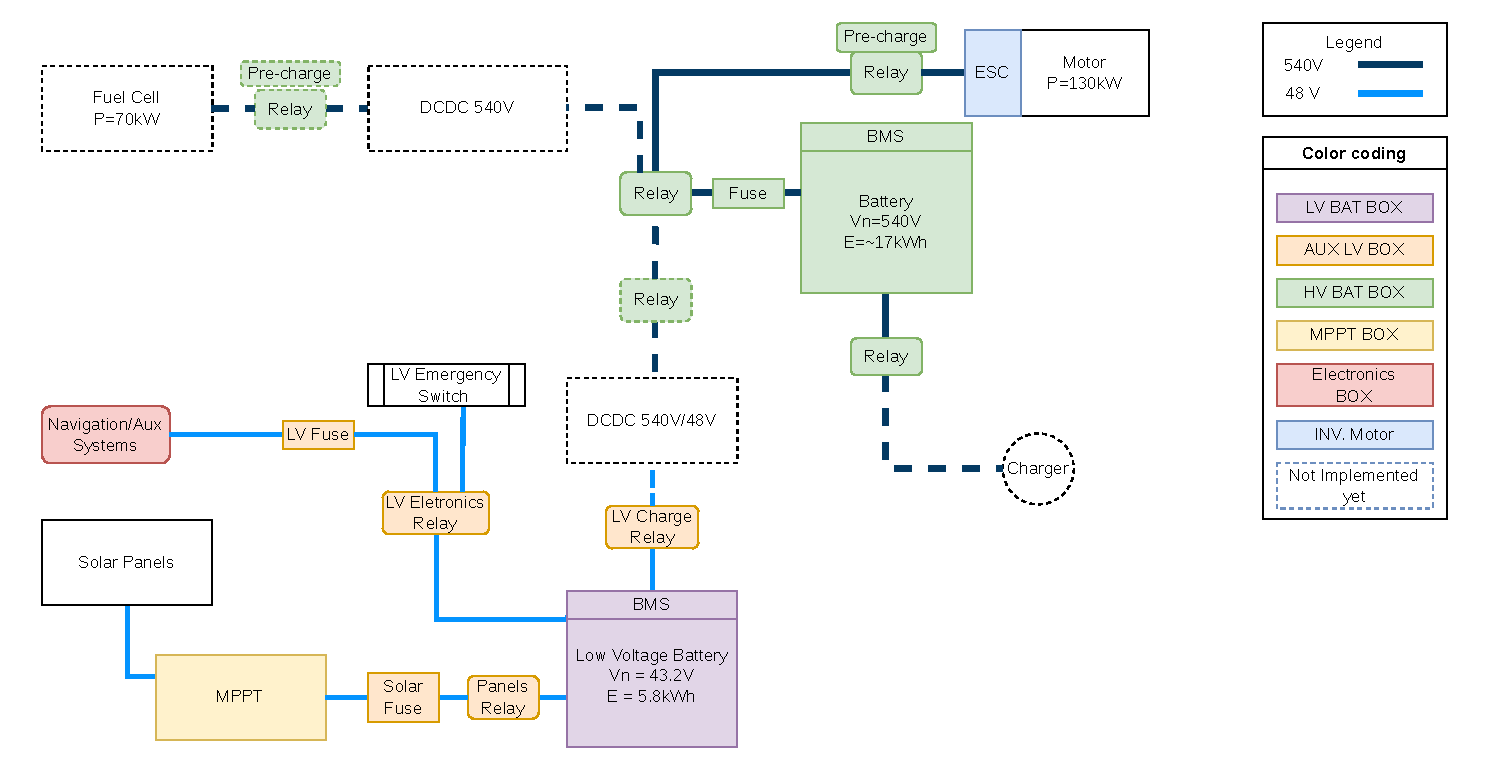
\includegraphics[width=0.92\linewidth,height=0.22\textheight,keepaspectratio]{Images/System/Sys_diagram.pdf}
    \caption{Simplified electrical architecture of SG01. Solar conversion serves the low-voltage auxiliary battery.}
    \label{fig:architecture}
\end{figure}

\subsection{Photovoltaic installation and battery}

The present array uses 140 Maxeon Gen~3 cells in ten panels built by the team, with a total active area of $2.171~\mathrm{m}^2$. At standard test conditions the theoretical peak is $526.4~\mathrm{W}$. Unused deck area could raise that to about $977~\mathrm{W}$. Each cell string seen by one charger is specified from 20 to 40 series cells and is optimized for 35 cells (Table~\ref{tab:pv}). Electroluminescence inspection was used before installation to reject cracked cells.

The onboard low-voltage pack is a 12s28p assembly of Samsung INR21700-50G cells (43.2~V nominal, 50.4~V maximum, 30~V minimum, 135.8~Ah). It was carried over from another boat and is heavier than SG01 needs. Autonomy estimates therefore also use the smaller 12s7p pack from São Rafael 03 (35~Ah, 1512~Wh). A 12s1p pack (5.14~Ah) was used only to shorten laboratory charge tests. Both TSB packs accept more current than a string can deliver (short-circuit current $6.37~\mathrm{A}$), so on the boat the panel, not the battery, sets the constant-current phase.

\begin{table}[!t]
    \centering
    \caption{String operating points at the MPP (Maxeon Gen~3).}
    \label{tab:pv}
    \footnotesize
    \setlength{\tabcolsep}{3.5pt}
    \begin{tabular}{lcccc}
        \toprule
        String & $V_{\mathrm{mp}}$ & $I_{\mathrm{mp}}$ & $P_{\mathrm{mp}}$ & $V_{\mathrm{oc}}$ \\
        & (V) & (A) & (W) & (V) \\
        \midrule
        40 cells & 24.68 & 6.05 & 140 & 29.0 \\
        35 cells & 21.88 & 6.05 & 122 & 25.4 \\
        20 cells & 12.34 & 6.05 & 70 & 14.5 \\
        \bottomrule
    \end{tabular}
\end{table}

With 526~W available, the oversized pack needs about 11~h to charge from empty and the 1512~Wh pack about 2~h~53~min. At 1000~W of auxiliary load the 1512~Wh pack lasts 1~h~30~min with no sun and 3~h~12~min if the present array delivers its STC power, roughly doubling endurance. The larger pack stretches from 5~h~51~min to 12~h~21~min. These figures are upper bounds: marine irradiance is below $1000~\mathrm{W/m}^2$ for most of a day, which is why tracking losses matter.

\subsection{How fast the tracker must be}

Temperature on deck usually moves slowly. Irradiance does not. Roll and pitch change the incidence angle on a time scale set by the waves and by the hull. Hydrostatic data give metacentric heights $GM_L = 21.515~\mathrm{m}$ and $GM_T = 1.867~\mathrm{m}$. With ITTC radii of gyration of $0.25L$ in pitch and about $0.4B$ in roll ($L = 8~\mathrm{m}$, $B = 2.5~\mathrm{m}$)~\cite{ittc_seakeeping_2024,rao2011mechanical}, the undamped natural periods are $0.87~\mathrm{s}$ in pitch and $1.29~\mathrm{s}$ in roll. Wave energy is concentrated between roughly 1 and 30~s~\cite{newfrontiers2018}. Records taken with SG01 adrift show spectral peaks near $0.05~\mathrm{Hz}$ and $0.5~\mathrm{Hz}$.

The design target follows those periods: the operating point should be back at the MPP in under 1~s, and typically in under 0.5~s. A tracker that needs one or two seconds, which is what some integrated charge controllers specify, gives away energy on every wave.

\section{Choices for Algorithm, Topology, and Charging}
\label{sec:choices}

\subsection{Tracking method}

Partial shading can create extra local peaks~\cite{Comparison_PV_Array_MPPT_Techniques_2007}, but the dominant disturbance on this boat is a fast, nearly uniform change of irradiance. Four families were compared against that disturbance.

Constant-voltage control holds the panel near a fixed fraction of the open-circuit voltage, often 71--78\%~\cite{Comparison_PV_Array_MPPT_Techniques_2007}. It is cheap and wrong whenever temperature or irradiance moves that fraction, and the open-circuit measurement interrupts production.

P\&O perturbs the panel voltage and keeps the direction that raises power~\cite{chermitti2012improvement,Look-Up-Table_VS_PeO}. It is the method used in most commercial chargers. It oscillates around the MPP, and a step that is too coarse wastes power while a step that is too fine loses the point when the curve moves. A fast irradiance change can also be mistaken for the effect of the last perturbation, so the tracker walks away from the MPP~\cite{4112312,Comparison_PV_Array_MPPT_Techniques_2007}.

Incremental conductance uses $dP/dV = 0$ at the MPP, rewritten as $dI/dV = -I/V$~\cite{Intelligent_PV_Module_2006,Comparison_PV_Array_MPPT_Techniques_2007}. It can stop the steady-state dither and it behaves more cleanly when irradiance changes quickly~\cite{bendib_survey_mppt_methods}. The cost is extra tuning and a division on every sample.

A look-up table can apply a duty cycle in one cycle, but the table does not follow cell aging, and accuracy costs memory.

P\&O was implemented. Incremental conductance is the natural next algorithm on the same hardware; it was left out so that sensing, protection, and the charge state machine could be validated with a tracker whose failure modes are well known. The oscillation and divergence limits are handled by a small duty-cycle step, a power deadband, and a periodic voltage sweep that rejects local peaks.

\subsection{Why a synchronous boost stage}

Galvanic isolation is unnecessary between the deck panels and the low-voltage battery, and a transformer would add loss, volume, and cost~\cite{Review_Isolated_Non_isolated_DC_DC_Converters_MVDC_2021}. Among non-isolated stages, a buck converter cannot be used: even a 40-cell string has $V_{\mathrm{oc}} = 29~\mathrm{V}$, below the 30~V battery floor. Buck--boost, Cuk, SEPIC, and ZETA converters would tolerate a future change of string length, at the price of more magnetics and a lower efficiency~\cite{Comparative_Analysis_Non_Isolated_DC_DC_Converters_Solar_PV_2021,Non_Isolated_DC_DC_Converters_MPPT_Controller_2021}. ZETA would be the fallback if step-up and step-down were both required, because the output is not inverted and the output current ripple is low. They are not required here.

The ideal boost relation is
\begin{equation}
    V_{\mathrm{out}} = \frac{V_{\mathrm{in}}}{1-D}, \qquad I_{\mathrm{in}} = \frac{I_{\mathrm{out}}}{1-D}.
    \label{eq:boost}
\end{equation}
With inductor resistance, MOSFET $R_{\mathrm{DS(on)}}$, and a diode drop $V_d$, the output falls by approximately $V_d$ plus resistive terms in the numerator. At this voltage a Schottky drop of 0.3--0.7~V is a large fraction of the loss budget. Replacing the diode with a second MOSFET (Fig.~\ref{fig:sync}) removes that term and leaves conduction loss $I^2 R_{\mathrm{DS(on)}}$~\cite{lee_high-efficiency_2019}. Literature efficiencies for a well-designed boost stage reach the high nineties~\cite{Review_Isolated_Non_isolated_DC_DC_Converter_PV_Application_2018}; the specification for this board was only $>90\%$, with a measured target well above that.

\begin{figure}[!t]
    \centering
    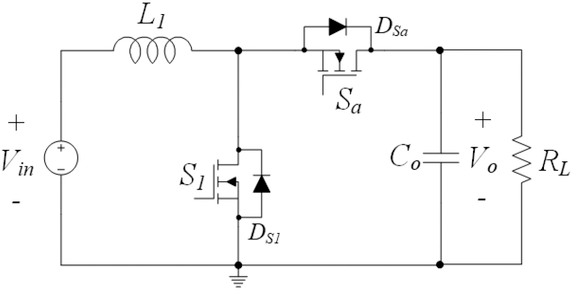
\includegraphics[width=0.72\linewidth]{Images/Implementation/Conventional-synchronous-boost-converter.png}
    \caption{Synchronous boost stage. The diode of the classical boost is replaced by a controlled MOSFET~\cite{lee_high-efficiency_2019}.}
    \label{fig:sync}
\end{figure}

\subsection{Battery charge profile}

The panel current is below half of the maximum charge current of either TSB pack, and the pack is not expected to see more than about 20 cycles per year. Multi-stage lithium profiles that try to shorten charge time are therefore unnecessary~\cite{Charging_Algorithms_Lithium_Ion_Batteries_Overview_2012,Review_Different_Charging_Techniques_Lithium_Polymer_Battery_2015}. CC--CV is used. While the battery voltage is below the limit, the tracker extracts maximum panel power, with a current limit above it. At the voltage limit the tracker is replaced by a proportional loop that holds the battery voltage and lets the current fall. Charging stops below a cutoff current.

\subsection{What the catalogue does not provide}

Integrated controllers such as the BQ24650, MAX20801, and SPV1040 do not support a 48~V lithium rail at the required current. The LT8491 does, and it already implements P\&O and CC--CV, but its tracking time is 1--2~s and its interface is I\textsuperscript{2}C rather than the vessel CAN bus. Complete chargers were no closer. The Genasun GVB-8-Li-CV already used by TSB is efficient (typically 96--99\%) and tracks at about 15~Hz, but it has no communication, no adjustable set-points, and costs about 240~\texteuro{}. Victron's SmartSolar MPPT 100/20 is a buck converter and wants a higher panel voltage than these short strings provide. An open design (Reboost) uses a GaN boost stage but depends on costly or discontinued parts. None of the reviewed units combine a boost stage, a sub-second tracker, configurable CC--CV limits, and the team's CAN protocol at a cost that can be repeated four times on one boat.

\section{Implementation}
\label{sec:impl}

\subsection{Power stage}

The switching frequency is 100~kHz: high enough to shrink the inductor, low enough that hard-switched GaN loss stays acceptable. Output voltage ripple is limited to $0.1~\mathrm{V}$ so that electronics sharing the battery rail are not disturbed, and input ripple to $0.5~\mathrm{V}$ so that the voltage sample used by P\&O is meaningful.

Continuous conduction sets a floor on inductance. With ripple factor $r = \Delta I_L / I_{L,\mathrm{avg}}$, the inductance that satisfies the ripple at a given duty cycle is largest at $D = 1/3$:
\begin{equation}
    L = \frac{4}{27}\,\frac{V_{\mathrm{out}}}{I_{\mathrm{out}}\, r\, f_{\mathrm{sw}}}.
    \label{eq:L}
\end{equation}
At $50.4~\mathrm{V}$, $10~\mathrm{A}$, and $r = 2$ (the continuous-conduction boundary) this is only $3.7~\mu\mathrm{H}$. A ripple factor of 0.4 raises it to $19~\mu\mathrm{H}$. The built inductor is $68~\mu\mathrm{H}$ (Würth 74437529203680), which corresponds to $r \approx 0.11$. It is rated 16~A, with $10.3~\mathrm{m}\Omega$ DC resistance. Saturation is specified at 7.2~A for a 10\% drop and 10.6~A for a 30\% drop. The worst-case sum of string short-circuit current and half the ripple exceeds the 10\% figure, but that corner (open-circuit voltage and short-circuit current at once) does not occur, and the extra inductance keeps the ripple acceptable after a partial drop.

The same corner-frequency argument gives $250~\mu\mathrm{F}$ on the output for $0.1~\mathrm{V}$ ripple at 10~A and $D = 0.5$, and $100~\mu\mathrm{F}$ on the input for $0.5~\mathrm{V}$. LTspice comparisons of capacitor banks (Section~\ref{sec:sim}) selected two $56~\mu\mathrm{F}$, 63~V electrolytics at the input and five $100~\mu\mathrm{F}$, 100~V electrolytics at the output, plus $1~\mu\mathrm{F}$ and $100~\mathrm{nF}$ ceramics for the switching edges. Parallel parts cut ESR and share ripple current.

At 100~kHz and roughly 100~W, GaN is the device that minimizes $R_{\mathrm{DS(on)}}$ and switching energy~\cite{talat2024igbt}. The EPC23102 integrates the half-bridge and its gate driver: $5.2~\mathrm{m}\Omega$, 100~V, 35~A, in a package that can be cooled through the board. Shoot-through protection is internal, but the firmware still inserts dead time. With the 80~MHz timer, a dead-time code of 3 measures 32~ns (rise 19~ns, fall 22~ns). Codes 2 and 3 differ by about 0.01~percentage points of efficiency in simulation, so the margin is kept. Complementary 100~kHz PWM from an 80~MHz clock has 0.125\% duty-cycle steps. Version 1.1 added Schottky diodes across the GaN devices; with only 0.375\% of the period spent in dead time their measured benefit was negligible, and they were left off the final bill of materials.

\subsection{Sensing and processor}

The microcontroller is an STM32L476 (Cortex-M4F, 80~MHz, 1~MB flash, 128~kB RAM). A faster clock or a 16-bit ADC would improve duty-cycle and measurement resolution; this part was already standard in TSB, which shortened bring-up. It provides the CAN controller, complementary PWM with dead time, and three 12-bit ADCs. An independent watchdog resets the core if the control loop stops kicking it. The ADC is scanned and polled; each P\&O update averages the samples gathered since the previous update, about ten samples at 1~kHz.

Panel and battery currents use INA253A2 shunt amplifiers with PWM rejection, at $0.2~\mathrm{V/A}$. On a 3.0~V, 12-bit reference the current quantum is $3.7~\mathrm{mA}$. Voltages use dividers of $10/210$, a quantum of $15~\mathrm{mV}$. Board and transistor temperature use NTC thermistors and the usual $B$-parameter equation; the transistor sensor also drives a comparator that turns the half-bridge off above a hardware threshold. A footprint for a TSL2591 light sensor is on the board but was not populated: the device saturates outdoors and does not match the solar spectrum. A better irradiance input is a small cell of the same type, read as a temperature-corrected short-circuit current.

\subsection{Firmware}

A 1~ms tick schedules two main jobs. The measurement job converts ADC codes, applies the calibration described in Section~\ref{sec:results}, and latches a fault if a limit is crossed. Faults hold the converter off for 5~s and are then rechecked, so a noise spike does not become a permanent shutdown. The power job updates the state machine of Fig.~\ref{fig:sm} and writes the duty cycle.

\begin{figure}[!t]
    \centering
    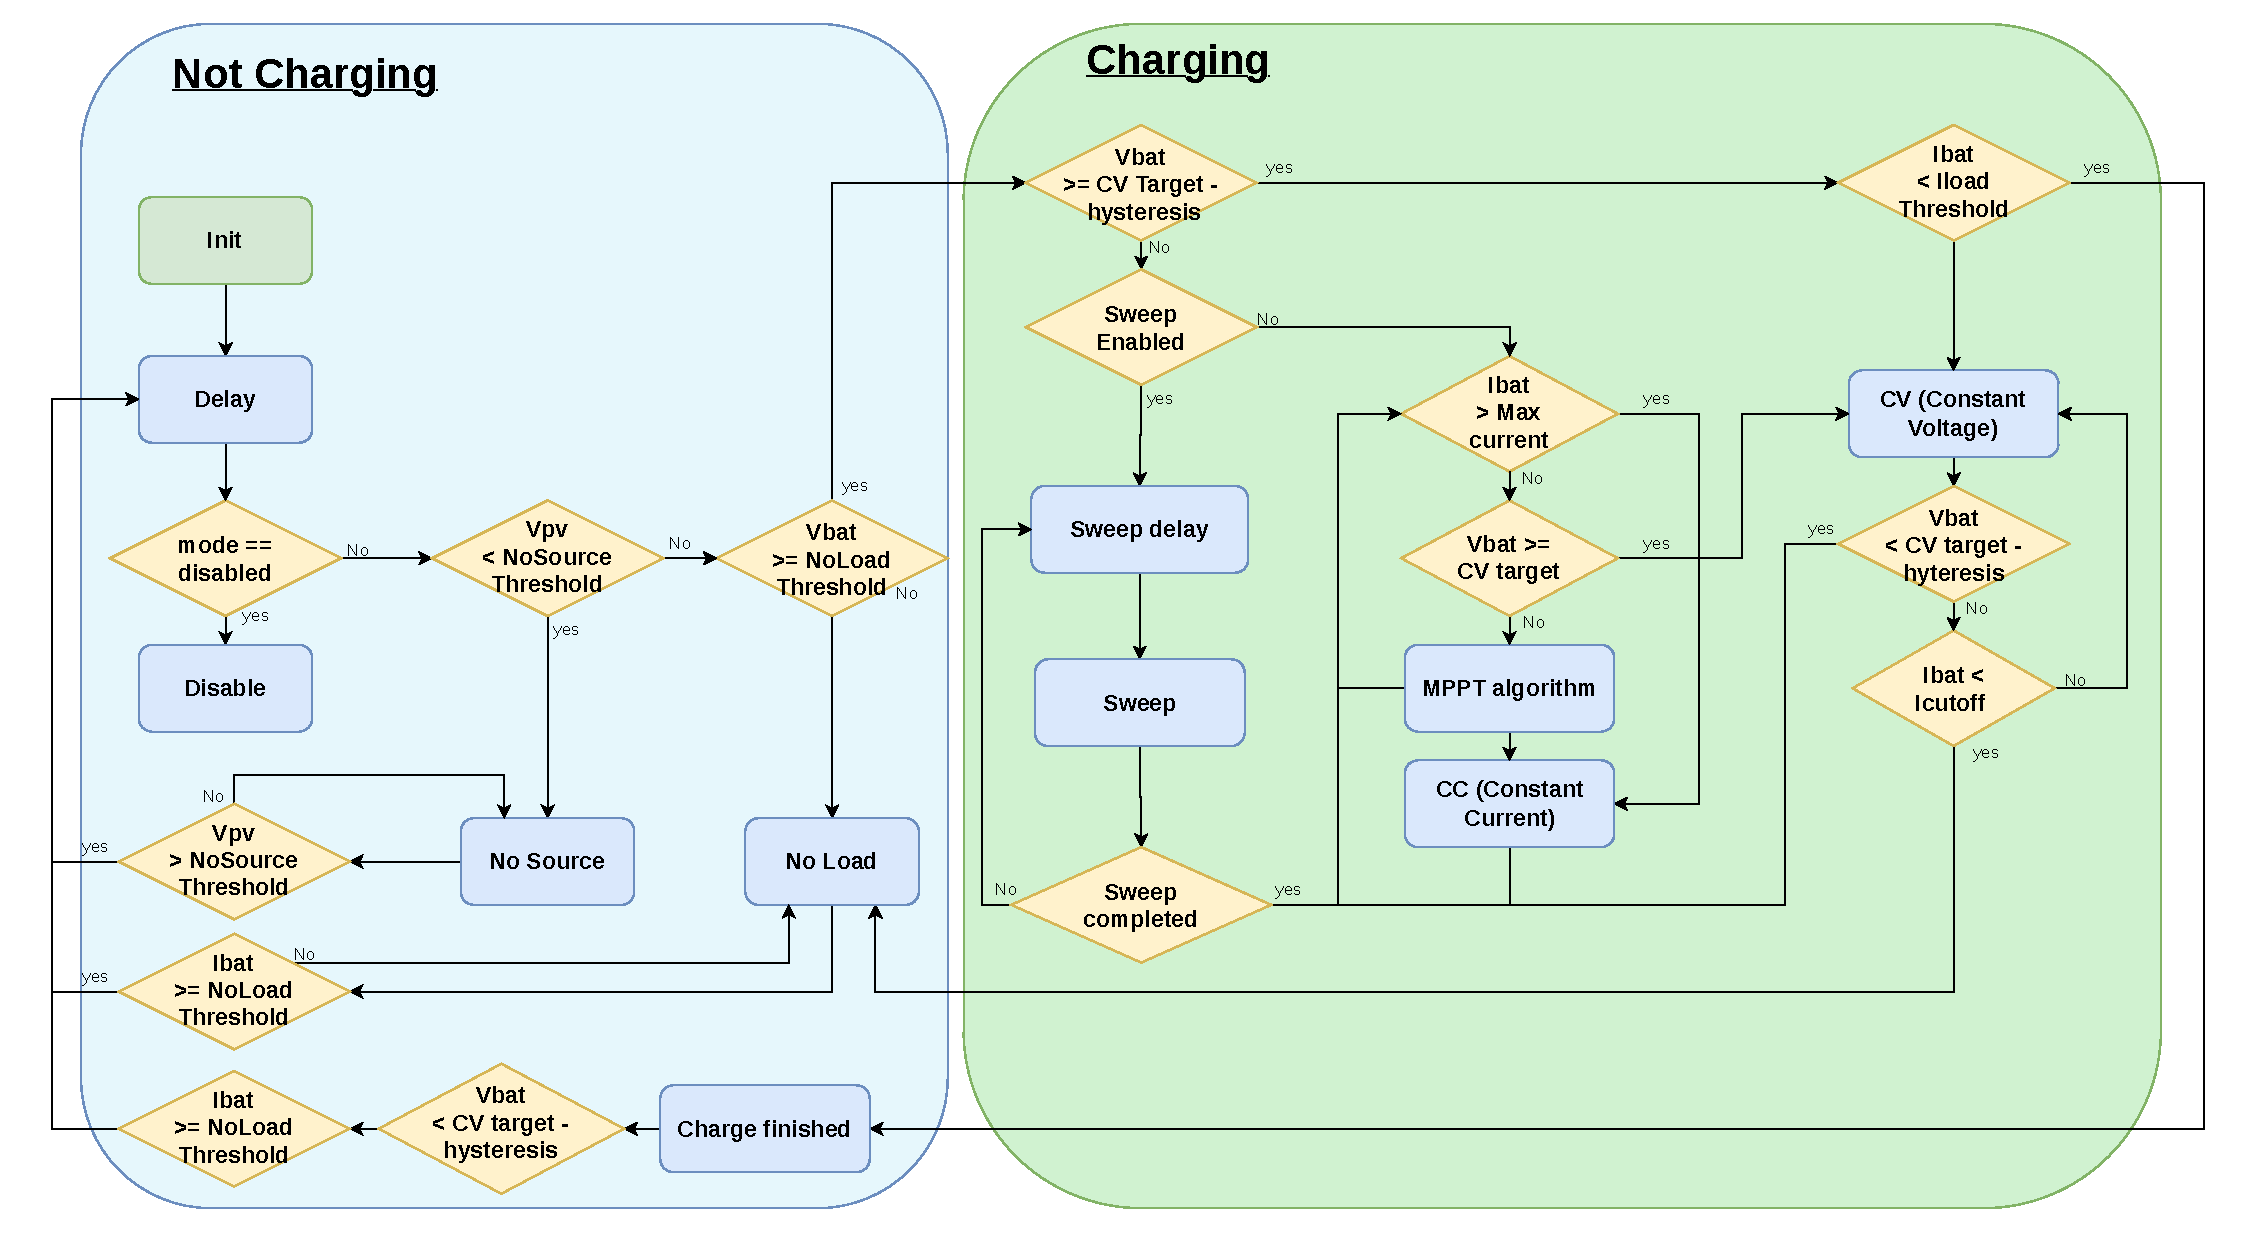
\includegraphics[width=\linewidth,height=0.30\textheight,keepaspectratio]{Images/Implementation/MPPT_state_machine.drawio.pdf}
    \caption{Charge state machine. Tracking runs only while both the string and the battery are present and inside their limits.}
    \label{fig:sm}
\end{figure}

Idle states cover a start-up delay, a disabled bridge, a missing panel, a missing battery, and a finished charge. In the last two, the output is held at the maximum battery voltage so that reconnecting the pack does not demand a separate precharge path. Charge states are a voltage sweep (to step over local maxima), the P\&O loop, a current-limit loop, and a voltage-limit loop. Sweep steps are separated by a short delay so that each sample is taken after the LC transient.

Set-points live in internal flash, written by an EEPROM emulation library with wear leveling across ten pages. A full configuration is a handful of 16-bit values, so endurance is not a practical limit. The linker script keeps program code out of that region.

Telemetry uses the team CAN 2.0A layout: 5~bits of device identifier and 6~bits of message identifier, with the top three message bits selecting which of up to eight trackers is speaking. Each tracker publishes battery-side, panel-side, and auxiliary frames. A serial framing format (start byte, identifiers, length, payload, checksum, end byte) carries the same measurements plus the configuration records, so a laptop can set current and voltage limits, P\&O parameters, and CAN identifiers without a CAN adapter. A Qt application plots the operating point against a family of power--voltage curves and shows the CC--CV trajectory.

\section{Simulation}
\label{sec:sim}

\subsection{Converter}

The string was represented in LTspice by a single-diode five-parameter model~\cite{LOBRANO2013894}, with parameters fitted to $V_{\mathrm{oc}}$, $I_{\mathrm{sc}}$, and the MPP. The battery was a voltage source in series with its resistance. Manufacturer switch and passive models were used, including the measured rise, fall, and dead times.

Five points along a CC--CV trajectory of a 35-cell string were simulated. Capacitor banks all lost well under 1\% on the high-power points; the chosen pair (two $56~\mu\mathrm{F}$ at the input, five $100~\mu\mathrm{F}$ at the output) was the best among parts that were actually in stock. Inductors from $22~\mu\mathrm{H}$ to $100~\mu\mathrm{H}$ were then compared with that capacitor set. Smaller cores waste less DC resistance but produce several amperes of current ripple; $100~\mu\mathrm{H}$ increases loss. At $68~\mu\mathrm{H}$ the inductor ripple stays near 1--2~A (Table~\ref{tab:ripple}) and the loss on the four high-power points is 0.58--0.75\%. The fifth point, deep in the constant-voltage tail, loses 3.5\% because the processed power is small. Both voltage ripples are inside the $0.1~\mathrm{V}$ and $0.5~\mathrm{V}$ specifications. A battery-voltage sweep shows the expected trend: efficiency falls as the conversion ratio rises.

\begin{table}[!t]
    \centering
    \caption{LTspice ripple and loss with $L = 68~\mu\mathrm{H}$, two $56~\mu\mathrm{F}$ input capacitors, and five $100~\mu\mathrm{F}$ output capacitors.}
    \label{tab:ripple}
    \footnotesize
    \setlength{\tabcolsep}{3.2pt}
    \begin{tabular}{ccccc}
        \toprule
        Point & $\Delta V_{\mathrm{bat}}$ & $\Delta V_{\mathrm{pv}}$ & $\Delta I_L$ & Loss \\
        & (V) & (V) & (A) & (\%) \\
        \midrule
        1 & 0.041 & 0.015 & 0.98 & 0.58 \\
        2 & 0.049 & 0.021 & 1.71 & 0.68 \\
        3 & 0.053 & 0.024 & 1.96 & 0.75 \\
        4 & 0.041 & 0.022 & 2.01 & 0.67 \\
        5 & 0.030 & 0.022 & 1.96 & 3.46 \\
        \bottomrule
    \end{tabular}
\end{table}

LTspice does not attribute the loss. An analytical model sums transistor conduction, switching and $C_{\mathrm{oss}}$ energy, dead-time reverse conduction, inductor DC loss plus AC loss from the manufacturer's REDEXPERT tool, capacitor ESR loss, gate-drive charge, shunt loss, and the 3.3~V and 5~V auxiliary rails:
\begin{align}
    P_{\mathrm{sw}} &= \tfrac{1}{2} V_{\mathrm{out}} I_{L} (t_r+t_f) f_{\mathrm{sw}} + \tfrac{1}{2} C_{\mathrm{oss}} V_{\mathrm{out}}^{2} f_{\mathrm{sw}}, \\
    P_{\mathrm{dead}} &= 2\, V_f I_{L}\, t_{\mathrm{dead}}\, f_{\mathrm{sw}}.
\end{align}
At the second operating point the model predicts $1.98~\mathrm{W}$, or 98.5\% efficiency (Fig.~\ref{fig:loss}). Inductor copper is the largest term. GaN conduction is about 24\% of the total and the capacitors about 24\%. Auxiliary electronics are comparable to the magnetics, which is why end-to-end efficiency and power-stage efficiency must be reported separately. Board copper is absent from the model and shows up later as a gap versus the bench.

\begin{figure}[!t]
    \centering
    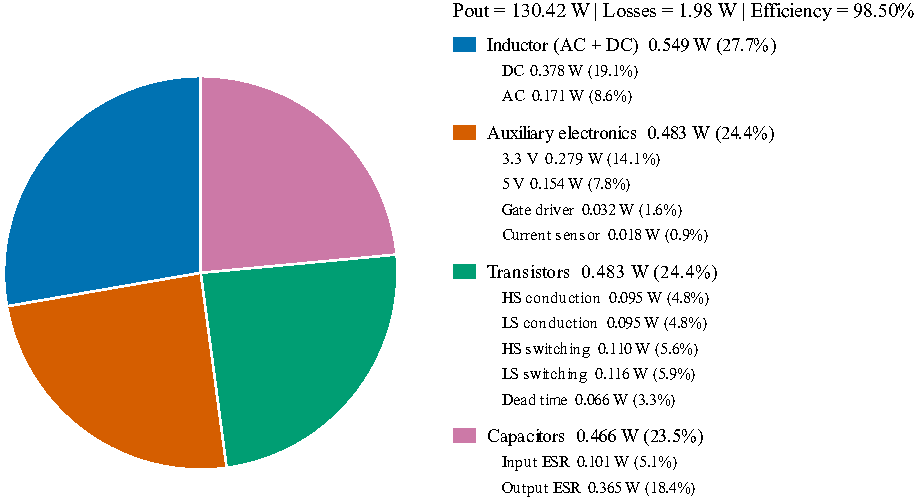
\includegraphics[width=0.95\linewidth,height=0.24\textheight,keepaspectratio]{Images/Implementation/fig_loss_breakdown.pdf}
    \caption{Analytical loss split at operating point 2. Total loss $1.98~\mathrm{W}$ (98.5\%).}
    \label{fig:loss}
\end{figure}

\subsection{Tracker tuning}

A Simulink model of the boost stage, the 35-cell string, and the SG01 battery was used to choose the P\&O step before the hardware existed. The plant model is a diode boost rather than the synchronous stage; efficiency is not the quantity under test. Sensor noise is included, and the algorithm receives a 10-sample average.

A sweep of the steady-state duty cycle shows that irradiance, from high sun to heavy cloud, moves the optimum by about 3\% of duty cycle, whereas temperature from cold panels to a hot deck moves it by about 9\%. The slow disturbance is therefore the one that demands range, and the fast disturbance is the one that demands a short step. At 100~Hz, fifty steps fit inside the 0.5~s budget, so a 0.18\% step would cross a 9\% move in time. That step disappears into the noise. Steps of 0.5\%, 1\%, and 2\% were compared on a $10~^\circ\mathrm{C/s}$ ramp and on a step from $25~^\circ\mathrm{C}$ to $85~^\circ\mathrm{C}$. The 0.5\% step was accurate and, on the large temperature step, took about 1~s to enter a $\pm 5\%$ power band, which is the specification limit. Larger steps arrived sooner and dithered more. Irradiance steps from 1000 to $200~\mathrm{W/m}^2$ were recovered almost immediately at every step size, consistent with the smaller duty-cycle travel. A step between 0.5\% and 1\% was carried to the bench.

\section{Experimental Results}
\label{sec:results}

Three boards were fabricated (Eurocircuits) and soldered by hand. The bill of materials is about 90~\texteuro{} and the bare board 3--35~\texteuro{}, so a finished charger is about 125~\texteuro{}, against 240~\texteuro{} for the Genasun unit it is intended to replace. Version 1 had a misplaced connector, a programming header without 5~V, and swapped UART pins. Version 1.1 fixed those errors, added the optional Schottky diodes and a fan connector, and was the board used for most of the numbers below. Version 1.2 moved the sense filters next to the ADC pins and fitted the extra ceramics that the noise tests required. The outdoor charge used version 1.2.

\subsection{Measurement error and switching noise}

Voltage readings from 0 to 51~V had mean absolute errors of 60~mV on the battery divider and 112~mV on the panel divider before correction. The error is close to linear, and subtracting it in firmware reduced both to about 29~mV. Current errors were 100~mA on the battery shunt and 8.5~mA on the panel shunt; battery-current calibration reduced the mean error to 5.3~mA. Per-board calibration is reasonable in a thesis prototype and tedious in a fleet, so the production path is still tighter resistors or a one-point trim.

Early runs tripped overcurrent protection on switching spikes. The input current wandered between about 4 and 12~A during those events. The output ceramic network was a single $1~\mu\mathrm{F}$, against ten $1~\mu\mathrm{F}$ parts on the GaN evaluation board. Adding nine $1~\mu\mathrm{F}$ capacitors cut the input-current excursion from 1.8~A to 640~mA and the input-voltage excursion from 2.0~V to 350~mV. Six additional $100~\mathrm{nF}$ capacitors brought the input-current spike to about 290~mA. The Schottky diodes did not improve the spectrum enough to justify their cost. A conducted scan from 22~V into a $10~\Omega$ load at $D = 52.5\%$, and a second scan at no load with the output held at 50.4~V, stayed under the CISPR~25 Class~5 limits in the tabulated bands. The setup had no LISN and no shielded room, so this is an indication, not a certificate. Version 1.2, with the filters at the microcontroller, also cleaned the one-minute sense records that version 1.1 left noisy.

\subsection{Efficiency and temperature}

The bridge was run open-loop from a supply into a resistive load at the same CC--CV points used in simulation. Table~\ref{tab:eff} includes the 0.51~W drawn by the controller. End-to-end efficiency is 96.6--96.8\%. Removing the controller, and then the gate-drive overhead measured with the bridge switching at no load, puts the power stage near 97.4--98.2\%. That is about two points below the analytical 98.5\%, in line with copper and layout loss that the spreadsheet omitted, and well above the 90\% floor.

\begin{table}[!t]
    \centering
    \caption{Measured efficiency. The last two columns subtract the 0.51~W controller rail and the additional no-load switching overhead.}
    \label{tab:eff}
    \footnotesize
    \setlength{\tabcolsep}{2.6pt}
    \begin{tabular}{lcccc}
        \toprule
        Case & $P_{\mathrm{in}}$ & $P_{\mathrm{out}}$ & $\eta$ & $\eta$ stage \\
        & (W) & (W) & (\%) & (\%) \\
        \midrule
        1 & 127.4 & 123.4 & 96.8 & 97.6 \\
        2 & 129.1 & 124.7 & 96.6 & 97.4 \\
        3 & 127.5 & 123.2 & 96.6 & 97.4 \\
        4 & 73.1 & 70.8 & 96.8 & 98.2 \\
        \bottomrule
    \end{tabular}
\end{table}

With the tracker closed and a photovoltaic supply emulator, efficiency rises with panel current until about 3~A and then declines slightly as switching loss grows. Longer strings are more efficient because they reduce $D$ in \eqref{eq:boost}. Raising the battery voltage at fixed panel voltage does the opposite.

After 10~min the inductor was the hottest part, near $43~^\circ\mathrm{C}$, with the adjacent electrolytics and the GaN devices a few degrees lower, matching the loss ranking. A three-hour run at the highest-power point leveled off after about 40~min in free air. Inside a closed box, as the chargers are mounted on the boat, temperatures leveled after about 60~min and the peak was $51.6~^\circ\mathrm{C}$. No fan is required at this power.

\subsection{Tracking and charging}

The emulator (Delta SM~1500-CP-30, photovoltaic mode, 35 cells, $25~^\circ\mathrm{C}$ unless temperature was the stimulus) fed the charger into the 12s7p pack. The final P\&O settings, after the sweep suggested by simulation, are a 1~kHz sample rate, a 50~Hz update, a 0.7\% duty-cycle step, and a 700~mW power deadband. The slower update relative to the 100~Hz Simulink cases leaves the 0.7\% step inside the 0.5--1\% window and keeps the dither inside the deadband.

Disconnecting the source or the load produced the corresponding idle states. With both connected, the machine sat in P\&O; raising irradiance until the output current hit a 2~A test limit moved it into current limit. On a real panel the sweep walked the voltage across the curve and then handed the peak to P\&O. The emulator occasionally overcurrent-tripped during a sweep, so sweep tests used the panel.

An irradiance staircase (1000 down to $200~\mathrm{W/m}^2$ in $200~\mathrm{W/m}^2$ steps every 2~s, then a single jump back) and a temperature staircase ($25~^\circ\mathrm{C}$ to $85~^\circ\mathrm{C}$ in $10~^\circ\mathrm{C}$ steps, then a single jump back) were applied over TCP. Fig.~\ref{fig:stairs} shows the measured power. Time to re-enter $\pm 5\%$ of the MPP power was under 100~ms on the irradiance steps and on the gradual temperature steps. The $85~^\circ\mathrm{C}$ to $25~^\circ\mathrm{C}$ jump, the case simulation had flagged as slowest, took about 200~ms. Average tracking accuracy was about 99\%, with the largest offset at $85~^\circ\mathrm{C}$, where residual sense noise is the likely cause. Both numbers meet the 1~s / 0.5~s requirement from Section~\ref{sec:system} with margin.

\begin{figure}[!t]
    \centering
    \begin{minipage}[t]{0.48\linewidth}
        \centering
        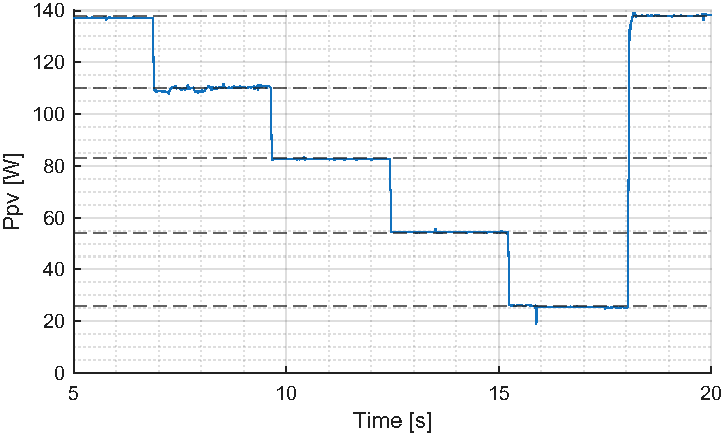
\includegraphics[width=\linewidth]{Images/LAB_res/irr_stairway.pdf}
        \centerline{\footnotesize (a)}
    \end{minipage}\hfill
    \begin{minipage}[t]{0.48\linewidth}
        \centering
        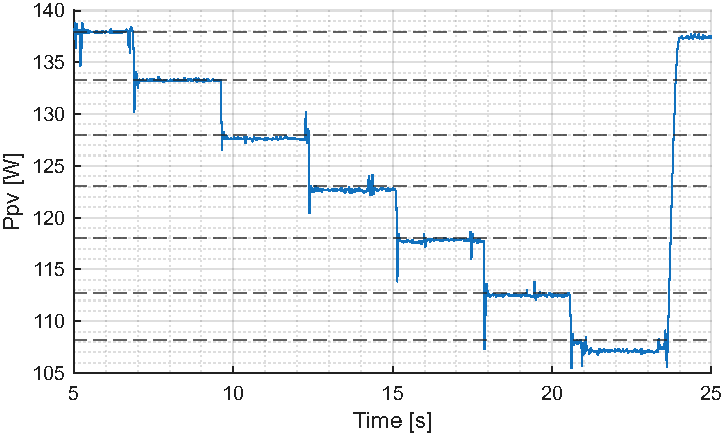
\includegraphics[width=\linewidth]{Images/LAB_res/temp_stairway.pdf}
        \centerline{\footnotesize (b)}
    \end{minipage}
    \caption{Closed-loop power during (a) the irradiance staircase and (b) the temperature staircase. The tracker stays on the moving MPP and recovers the large final step in a fraction of a second.}
    \label{fig:stairs}
\end{figure}

A full laboratory charge of the 12s1p pack reproduced CC--CV (Fig.~\ref{fig:charge}): P\&O held the panel at the MPP until the voltage limit, the current then decayed at constant voltage, and the machine entered the finished state. Outdoors, a 20-cell module under wind and two deliberate moves of the panel still produced a recognizable CC interval followed by CV. The outdoor run used revision 1.2. The charger has not yet been operated on SG01.

\begin{figure}[!t]
    \centering
    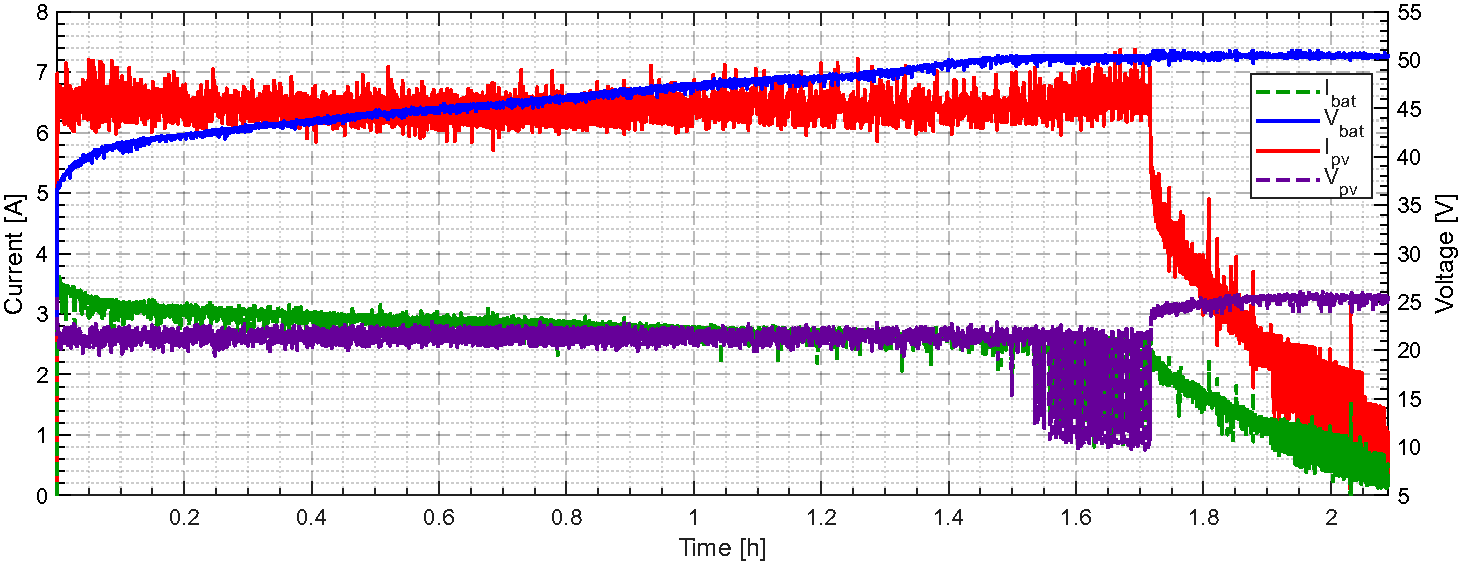
\includegraphics[width=0.95\linewidth,height=0.22\textheight,keepaspectratio]{Images/LAB_res/charging_test_lab.pdf}
    \caption{Laboratory charge of the 12s1p pack from the photovoltaic emulator. Constant current is the panel MPP; constant voltage follows once the cell limit is reached.}
    \label{fig:charge}
\end{figure}

Table~\ref{tab:vsreq} collects the quantities the project set out to hit. Efficiency, cost, and tracking time are met on the bench. The open items are a campaign on SG01 and a second algorithm on the same hardware.

\begin{table}[!t]
    \centering
    \caption{Requirements and what the prototype measured.}
    \label{tab:vsreq}
    \footnotesize
    \setlength{\tabcolsep}{3pt}
    \begin{tabular}{p{0.28\linewidth}p{0.30\linewidth}p{0.32\linewidth}}
        \toprule
        Item & Target & Result \\
        \midrule
        End-to-end efficiency & $>90\%$ & 96.6--96.8\% \\
        Power-stage efficiency & --- & 97.4--98.2\% \\
        Tracking time & $<1~\mathrm{s}$, typically $<0.5~\mathrm{s}$ & $<100~\mathrm{ms}$, worst $200~\mathrm{ms}$ \\
        Tracking accuracy & high & $\approx 99\%$ \\
        Unit cost & below the 240~\texteuro{} charger in use & $\approx 125$~\texteuro{} \\
        Enclosure temperature & no extra cooling & peak $51.6~^\circ\mathrm{C}$ \\
        Telemetry & vessel CAN, configurable limits & CAN and serial \\
        \bottomrule
    \end{tabular}
\end{table}

\section{Conclusion}

The auxiliary bus of a solar hydrofoil does not need a high-power tracker. It needs a repeatable boost charger that follows deck irradiance on a sub-second scale, speaks the boat's CAN protocol, and survives a student-built assembly. Vessel measurements set that scale at about 0.5--1~s. A synchronous 100~kHz boost stage and a tuned P\&O loop meet it: 96.6--96.8\% from panel to battery, about 97--98\% in the power stage, tracking usually inside 100~ms and inside 200~ms in the worst tested step, at roughly 99\% of available power. Component temperatures saturate near $52~^\circ\mathrm{C}$ in an enclosure. The parts cost about half of the commercial charger now fitted, and the set-points are configurable.

The prototype is not yet a fleet design. Current-sense error still depends on a per-board fit, the loss model misses layout resistance, and there is no campaign on the vessel or across several battery voltages and string lengths. Interleaving the four chargers that already share the battery would cancel output ripple and allow a smaller capacitor bank. A 16-bit ADC and a faster PWM clock would tighten the 0.7\% step. Incremental conductance, or a variable-step P\&O, should be run on the same board against the staircases already scripted, and a matched-cell irradiance sensor would make that comparison quantitative.

\bibliographystyle{IEEEtran}
\bibliography{../Thesis/Bibliography/Bibliography}

\end{document}
